%---------------------------------------------------------------------
%
%                          Cap�tulo 3
%
%---------------------------------------------------------------------
%
% 03Edicion.tex
% Copyright 2009 Marco Antonio Gomez-Martin, Pedro Pablo Gomez-Martin
%
% This file belongs to the TeXiS manual, a LaTeX template for writting
% Thesis and other documents. The complete last TeXiS package can
% be obtained from http://gaia.fdi.ucm.es/projects/texis/
%
% Although the TeXiS template itself is distributed under the 
% conditions of the LaTeX Project Public License
% (http://www.latex-project.org/lppl.txt), the manual content
% uses the CC-BY-SA license that stays that you are free:
%
%    - to share & to copy, distribute and transmit the work
%    - to remix and to adapt the work+
%
% under the following conditions:
%
%    - Attribution: you must attribute the work in the manner
%      specified by the author or licensor (but not in any way that
%      suggests that they endorse you or your use of the work).
%    - Share Alike: if you alter, transform, or build upon this
%      work, you may distribute the resulting work only under the
%      same, similar or a compatible license.
%
% The complete license is available in
% http://creativecommons.org/licenses/by-sa/3.0/legalcode
%
%---------------------------------------------------------------------


\begin{FraseCelebre}
\begin{Frase}
%Si quieres ser le�do m�s de una vez, no vaciles en borrar a menudo.
%Rem tene, verba sequentur (Si dominas el tema, las palabras vendr�n solas)
\end{Frase}
\begin{Fuente}
%Horacio
%Cat�n el Viejo
\end{Fuente}
\end{FraseCelebre}


\chapter{Especificaci\'on del protocolo de comunicaci\'on}
\label{cap3}
\label{cap:especificacion}

%-------------------------------------------------------------------
\section{Introducci\'on}
%-------------------------------------------------------------------
\label{cap3:sec:intro}
En este cap\'itulo se describen las diferentes decisiones tecnol\'ogicas involucradas en el proyecto y ver las decisiones tomadas en base a las necesidades para la realizaci\'on de este proyecto. La finalidad del proyecto es la conexi\'on entre 2 dispositivos, uno de ellos ejecuta el juego y el otro funciona como un dispositivo de entrada / mando para controlar el videojuego. 
Para conseguir esta comunicaci\'on entre ambos dispositivos es necesario plasmar la funcionalidad que se quiere dar y la posterior creaci\'on e implementaci\'on de un protocolo de red.


%-------------------------------------------------------------------
\section{Funcionalidad}
%-------------------------------------------------------------------

En los \'ultimos a\~nos se ha visto un aumento en la incorporaci\'on de elementos t\'actiles en los controladores de videojuegos. Empresas como Sony a\~nadieron una pantalla t\'actil en el Dualshock4, Nintendo con las consolas port\'atiles lleva varias generaciones a\~nadiendo pantallas t\'actiles a sus consolas y los dispositivos m\'oviles cada vez son m\'as usados para jugar a videojuegos.
Es por esto que en este proyecto, la comunicaci\'on entre 2 dispositivos ser\'a m\'as precisa y ser\'a entre un dispositivo en el cual se ejecuta el juego y un dispositivo m\'ovil que servir\'a como mando. Una de las principales diferencias entre un mando tradicional y un dispositivo m\'ovil es la pulsaci\'on de botones. El feedback recibido en la pulsaci\'on de una pantalla t\'actil es inexistente a no ser que no se especifique en la funcionalidad de la aplicaci\'on y debe ser lo suficientemente sutil como para no ser molesto a la hora de jugar.

Otras de las caracter\'isticas que tiene un dispositivo m\'ovil frente a un mando tradicional es el uso de gestos espec\'ificos. Una gran parte de estos gestos son utilizados de manera natural ya que son asociados al uso de dispositivos m\'oviles. 

Al usar un dispositivo m\'ovil, tenemos a nuestra disposici\'on una pantalla que nos permite a\~nadir im\'agenes, videos o incluso gameplay como lo hac\'ia Nintendo con su consola WiiU.

Con estas caracter\'isticas contempladas, las principales funcionalidades que debe tener este proyecto son:

\begin {itemize}
\item Env\'io de pulsaciones en pantallas t\'actiles.
\item Env\'io de im\'agenes est\'aticas.
\item Env\'io de im\'agenes de manera constante, simulando un streaming de video.
\item El uso de vibraci\'on como feedback de la pulsaci\'on de la pantalla.
\end {itemize}

%-------------------------------------------------------------------
\section{Protocolo de comunicaci\'on entre juego y dispositivo de entrada}
%-------------------------------------------------------------------

Un protocolo de comunicaci\'on es un sistema de reglas que permiten a 2 o m\'as dispositivos comunicarse entre ellos. Estas reglas se establecen para permitir la transmisi\'on de datos y la forma en la que la informaci\'on debe ser procesada. Cada mensaje tiene un significado exacto destinado a obtener una respuesta de un rango de posibles respuestas predeterminadas para esa situaci\'on en particular. Una de las caracter\'isticas principales de un protocolo de comunicaci\'on es que ambas partes tienen que acordar los mensajes que se van a enviar y a recibir. 

En este proyecto ambos dispositivos env\'ian y reciben mensajes por lo que no puede definirse un servidor y un cliente, sin embargo se puede hacer una distinci\'on entre qui\'en env\'ia los botones que se han pulsado y qui\'en ejecuta el juego. El criterio utilizado para este proyecto ha sido el de un sistema \textbf{\textit{little-endian}}. Al inicio de la comunicaci\'on, el dispositivo encargado de ejecutar el juego debe quedarse a la escucha en un puerto asignado a la espera de un primer mensaje. El tama\~no de este mensaje es de 8 bytes y su estructura es la siguiente:

\begin {itemize}
\item Los 4 primeros bytes son un n\'umero de tipo \textit{int} que simboliza el ancho del dispositivo m\'ovil.
\item Los 4 \'ultimos bytes son un n\'umero de tipo \textit{int} que simboliza el alto del dispositivo m\'ovil.
\end {itemize}

\begin{table}[h!]
\centering
\begin{tabular}{|l|l|l|} 
\hline
Bits                    & 0-31                   & 32-63                   \\
\hline
\multicolumn{1}{|c|}{0} & \multicolumn{1}{c|}{Ancho} & \multicolumn{1}{c|}{Alto}  \\
\hline
\end{tabular}
\caption{Primer mensaje del controlador al ejecutor de juego}
\label{table:2}
\end{table}


La comprobaci\'on que se realiza en este mensaje es si se reciben 8 bytes en el lado del dispositivo que ejecuta el juego.

Una vez la conexi\'on se ha establecido correctamente, el dispositivo que ejecuta el juego env\'ia al controlador la duraci\'on de la vibraci\'on que debe realizar para que el usuario reciba un feedback h\'aptico. Este mensaje contiene un \textit{int} de 4 bytes que representa el tiempo que debe durar la vibraci\'on en milisegundos.

\begin{table}[h!]
\centering
\begin{tabular}{|l|c|} 
\hline
Bits                    & 0-31                 \\
\hline
\multicolumn{1}{|c|}{0} & Tiempo de vibraci\'on  \\
\hline
\end{tabular}
\caption{Tiempo de vibraci\'on del dispositivo movil en milisegundos}
\label{table:2}
\end{table}

Tras el env\'io de este mensaje comienza un bucle de juego en el que ambos dispositivos intercambian mensajes de una manera no ordenada. El dispositivo que se encarga de ejecutar el juego env\'ia los siguientes mensajes:
\begin {itemize}
\item En caso de que se decida enviar im\'agen de manera constante, ya sea en forma de streaming de video o una im\'agen est\'atica, esta im\'agen es comprimida en formato \textbf{\textit{PNG}}.
\item Se env\'ia el flag de vibraci\'on al controlador. Este flag es un \textit{int} de 4 bytes cuyo valor tiene que ser 0 para que vibre.
\end {itemize}

Adem\'as de enviar estos mensajes, el dispositivo encargado de ejecutar el juego recibir\'a mensajes de 9 bytes cada uno cuya estructura ser\'a:
\begin {itemize}
\item El primer byte es el tipo de la pulsaci\'on. El valor 0 indica el comienzo de la pulsaci\'on y el valor 1 indica el fin de la pulsaci\'on.
\item Los siguentes 4 bytes representan un \textit{int} cuyo valor indica la posici\'on X de la pantalla del dispositivo m\'ovil donde se ha pulsado el bot\'on.
\item Los \'ultimos 4 bytes representan un \textit{int} cuyo valor indica la posici\'on Y de la pantalla del dispositivo m\'ovil donde se ha pulsado el bot\'on.
\end {itemize}

\begin{table}[h!]
\centering
\begin{tabular}{|l|c|c|c|} 
\hline
Bits                    & 0-7               & 8-39                            & 40-71                            \\ 
\hline
\multicolumn{1}{|c|}{0} & Tipo de pulsaci\'on & \multicolumn{1}{l|}{Posici\'on X} & \multicolumn{1}{l|}{Posici\'on Y}  \\
\hline
\end{tabular}
\caption{Pulsaci\'on enviada desde el dispositivo m\'ovil al ejecutor del juego}
\label{table:2}
\end{table}

Para el cierre ordenado de la comunicaci\'on desde el dispositivo m\'ovil se env\'ia un mensaje de tama\~no 1 byte que tiene el valor 2. La recepci\'on de este mensaje hace que el dispositivo que ejecuta el juego env\'ie 1 byte con el valor 1 al dispositivo m\'oviles y ambos cierran la conexi\'on. Estos mensajes puedes enviarse y recibirse en cualquier momento en caso de que sucediese cualquier error durante la comunicaci\'on. Para la detecci\'on de una p\'erdida de conexi\'on entre el dispositivo m\'ovil y el dispositivo que ejecuta el juego, este dispone de un tiempo m\'aximo en el que si no se reciben mensajes se finaliza la conexi\'on (Time Out).

\begin{figure}[h]

\centering
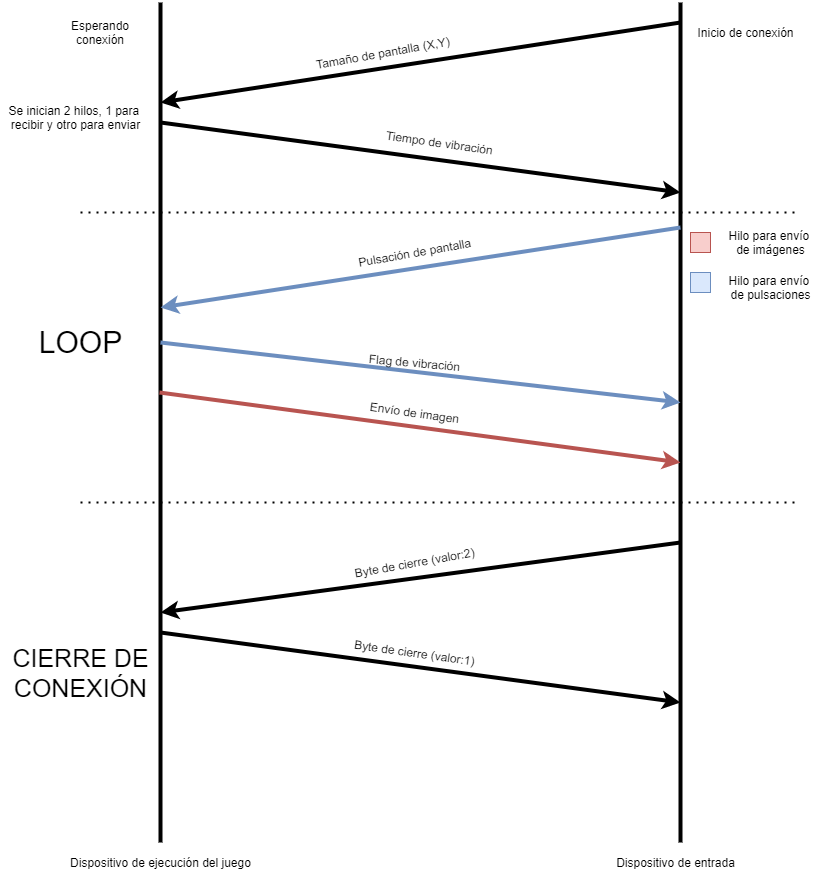
\includegraphics[width=0.9\textwidth]{./Imagenes/Bitmap/Arquitectura}
\caption{Diagrama del protocolo de comunicaci\'on entre ambos dispositivos}
\end{figure}



% Variable local para emacs, para  que encuentre el fichero maestro de
% compilaci�n y funcionen mejor algunas teclas r�pidas de AucTeX
%%%
%%% Local Variables:
%%% mode: latex
%%% TeX-master: "../ManualTeXiS.tex"
%%% End:
